\documentclass[a4paper,conference]{IEEEtran}
\IEEEoverridecommandlockouts
\usepackage{cite}
\usepackage{amsmath,amssymb}
\usepackage{booktabs}
\usepackage{graphicx}
\usepackage{url}
\usepackage{array}
\usepackage{placeins}
\usepackage{tikz}
\usetikzlibrary{arrows.meta, positioning}
\begin{document}
\title{Web-Based Liveness Detection Using Adaptive Temporal Multi-Cue Feature Fusion}

\author{\IEEEauthorblockN{Hanrocky Halim}
\IEEEauthorblockA{\textit{School of Computing, Telkom University}\
Bandung, Indonesia\\
hanrocky@student.telkomuniversity.ac.id}}

\maketitle
\begin{abstract}
Face presentation attack detection (PAD) protects face authentication systems against printed photographs and replayed videos. This paper compares six video-based liveness configurations using RGB appearance, inter-frame motion, and facial landmark geometry on a processed MSU Mobile Face Spoofing Database (MSU-MFSD) split. The configurations comprise RGB CNN, motion CNN, RGB--motion fusion, RGB--geometry fusion, concatenation-based three-stream fusion, and adaptive three-stream fusion with temporal mean pooling. A subject-disjoint protocol and common validation-based threshold selection are used. On 1,027 test sequences, E5 achieves the highest accuracy (94.06\%) and lowest maximum species-level APCER (1.83\%), whereas E6 achieves the lowest BPCER (10.34\%) and species-aware ACER (9.38\%). Subject-level bootstrap intervals do not establish a reliable difference in accuracy or ACER between E5 and E6. All six models were trained once with seed 42; repeated-seed variability and cross-dataset generalization are not established. A separate API benchmark records median sequential latency of 175.18 ms over 50 successful requests; this is not a concurrent-capacity measurement.
\end{abstract}
\begin{IEEEkeywords}
face presentation attack detection, face liveness detection, multimodal fusion, facial geometry, temporal aggregation, MSU-MFSD
\end{IEEEkeywords}

\section{Introduction}
Face recognition is used in identity verification and access control, but a recognition pipeline can be deceived by a printed photograph or replayed video of a genuine user. Face presentation attack detection (PAD) distinguishes bona fide presentations from presentation attacks. The MSU Mobile Face Spoofing Database (MSU-MFSD) supports research on print and replay attacks in mobile face authentication scenarios \cite{wen2015ida}.

RGB appearance encodes texture and image-quality cues, temporal differences describe changes between adjacent frames, and facial landmark geometry provides a representation of facial structure and movement. Prior work has investigated geometric temporal dynamics \cite{chang2023geometry} and multimodal feature alignment and fusion \cite{chen2025mmfas}. These studies motivate a controlled comparison of appearance, frame-difference motion, and landmark-derived geometry.

The research question is: \emph{How do RGB appearance, temporal motion, facial-landmark geometry, and their fusion strategies affect the APCER--BPCER trade-off and model ranking under consistent validation-based threshold selection in a subject-disjoint MSU-MFSD evaluation?} The contributions are: (1) a comparison of six compact configurations; (2) an evaluation of concatenation-based fusion against adaptive modality weighting with temporal mean pooling; and (3) a metric-sensitive analysis using species-level APCER, BPCER, ACER, and subject-level bootstrap intervals. This is an intra-dataset study and does not establish cross-dataset generalization.

\section{Related Work}
\subsection{CNN-based face presentation attack detection}
Deep learning has become a dominant approach to face anti-spoofing because CNNs can learn discriminative visual cues beyond manually designed texture descriptors; the broader design space, including auxiliary supervision, domain generalization, and multimodal sensing, is reviewed by Yu \emph{et al.}~\cite{yu2023survey}. Wen \emph{et al.} introduced MSU-MFSD and used image distortion analysis to detect print and replay attacks~\cite{wen2015ida}. Later methods explored stronger visual representations. Liu \emph{et al.} combined binary classification with auxiliary depth and rPPG supervision, arguing that auxiliary signals can guide networks toward more informative spoof cues~\cite{liu2018aux}. Yu \emph{et al.} proposed central-difference convolutions to capture intensity and gradient patterns, and reported evaluations across multiple benchmarks~\cite{yu2020cdcn}. These methods provide context for E1, the RGB-only CNN baseline in this study. Unlike CDCN or auxiliary-supervision systems, E1 uses a compact conventional CNN and classifies the first sampled frame; therefore, it is a controlled baseline rather than a direct reimplementation of a state-of-the-art architecture. However, a frame-level representation cannot explicitly model
temporal variations or facial geometric consistency, motivating
the investigation of complementary motion and geometry cues
in subsequent experiments.

\subsection{Temporal and motion-based cues}
A single image can contain texture, reflection, moir\'e, and border cues, but temporal evidence can capture changes across a video. Yang \emph{et al.} proposed the Spatio-Temporal Anti-Spoofing Network (STASN), combining local spatial and global temporal cues~\cite{yang2019stasn}. Sun \emph{et al.} compared CNN, 3D convolution, CNN--LSTM, Conv-LSTM, and optical-flow-based streams, showing the relevance of explicit temporal modelling and stream fusion~\cite{sun2018temporal}. Residual spatiotemporal convolutional networks were also investigated as end-to-end video models for FAS~\cite{silva2023spatiotemporal}. These approaches are more temporally expressive than the frame-difference and mean-pooling design used here. E2 isolates absolute adjacent-frame differences, while E3 combines that motion stream with RGB appearance. Under the conventional aggregate APCER calculation, E2 and E3
achieve ACER values of 12.30\% and 9.25\%, respectively.
When considering the maximum APCER across attack species,
their species-aware ACER values are 18.90\% and 12.55\%,
respectively. This comparison suggests that motion features
are more useful in combination with RGB than alone in this
implementation; it does not establish that simple frame
differences outperform optical flow or learned
spatiotemporal architectures generally.

\subsection{Facial geometry and multimodal fusion}
Chang \emph{et al.} proposed Geometry-Aware Interaction Network (GAIN), using dense facial landmarks and spatiotemporal graph convolution to model normal versus abnormal presentation dynamics~\cite{chang2023geometry}. Their graph-based temporal representation differs from the 936-dimensional mean landmark-displacement descriptor and MLP used in E4--E6. The latter is a lightweight geometry feature, not a reproduction of GAIN. In our results, E4 achieves an aggregate APCER of 1.31\% but has a BPCER of 24.52\%. When the maximum APCER across attack species is considered, the APCER increases to 2.80\%. This illustrates that geometry fusion changes the error trade-off rather than improving every metric.

Multimodal FAS has also combined RGB with depth and infrared data. FaceBagNet uses multi-stream CNNs and modality-feature erasing~\cite{shen2019facebagnet}; Yu \emph{et al.} extended central-difference networks to RGB, depth, and infrared modalities~\cite{yu2020multimodal}; and mmFAS investigates multi-level alignment with switch-attention fusion~\cite{chen2025mmfas}. A separate dual-stream method fuses original images with bandpass-filtered representations~\cite{zeng2023bandpass}. These methods demonstrate that fusion design and complementary cues are active research directions, but their sensor inputs and protocols differ from this study. E5 concatenates RGB, motion, and landmark geometry features, whereas E6 uses learned scalar gates to weight these three features before temporal mean pooling. E5 yields the highest accuracy (94.06\%) and F1-score (96.13\%), whereas E6 achieves the lowest species-aware ACER (9.38\%) and BPCER (10.34\%). These results indicate different operating characteristics: E5 provides stronger overall classification accuracy and lower attack acceptance,
while E6 produces a more balanced error trade-off under the species-aware ACER criterion. Therefore, adaptive weighting shows potential in balancing complementary cues in this experiment, but the result should not be interpreted as a general superiority claim over attention-based fusion or
sensor-level multimodal systems.

\subsection{Evaluation and deployment context}
ISO/IEC 30107-3 provides testing and reporting considerations for biometric PAD \cite{iso30107}. Accordingly, this paper reports APCER and BPCER separately and defines a species-aware ACER using the maximum APCER among evaluated attack species. Standard classification metrics are also reported \cite{sokolova2009}. API latency is a separate operational measurement and is not equivalent to concurrent serving capacity.

\section{Methodology}
\subsection{Dataset and subject-disjoint protocol}
Experiments use the Kaggle release ``MSU-MFSD Processed into Frames'' \cite{kagglemsumfsd}; the underlying database is described by Wen \emph{et al.} \cite{wen2015ida}. Labels are 0 for REAL (bona fide) and 1 for ATTACK. Each sequence contains eight frames sampled with stride five; each frame is resized to $112\times112$. The split is subject-disjoint: 12 training subjects, three validation subjects, and 20 test subjects. Validation contains 160 sequences (42 REAL, 118 ATTACK); test contains 1,027 sequences (261 REAL, 766 ATTACK), including iPad replay, iPhone replay, and printed-photo attacks.

Non-geometry training contains 621 sequences. Geometry preprocessing retains 579 because sequences with fewer than six valid landmark frames are excluded. All 42 excluded training sequences are REAL: the REAL count decreases from 159 to 117, while the ATTACK count remains 462. This changes both sample size and class composition, confounding comparisons involving E4--E6. All 1,027 test sequences have eight valid geometry frames; missing-geometry fallback at test time was not evaluated.

\subsection{RGB and motion inputs}
E1 classifies the first sampled RGB frame. E2 computes absolute adjacent-frame differences,
\begin{equation}
\mathbf{M}_t=|\mathbf{I}_{t+1}-\mathbf{I}_t|,\quad t=1,\ldots,7,
\end{equation}
and applies a CNN followed by temporal mean pooling. E3 uses separate RGB and motion branches, pools each branch over time, concatenates the pooled features, and classifies the fused representation.

\subsection{Facial geometry descriptor}
Facial landmarks are extracted using MediaPipe Face Landmarker. Each frame provides 468 two-dimensional points. Missing detections are interpolated, and training sequences are retained when at least six of eight frames contain valid detections. The resulting normalized sequence-level descriptor has 936 dimensions. The original implementation describes this descriptor as the mean adjacent-frame landmark displacement:
\begin{equation}
\mathbf{g}=\operatorname{vec}\left(\frac{1}{T-1}\sum_{t=1}^{T-1}(\mathbf{P}_{t+1}-\mathbf{P}_t)\right),
\label{eq:geometry}
\end{equation}
where $T=8$ and $\mathbf{P}_t\in\mathbb{R}^{468\times2}$. This compact descriptor is not a graph-convolution representation and is not a reproduction of GAIN \cite{chang2023geometry}.

\subsection{Fusion configurations}
E1 is an RGB CNN; E2 is a motion CNN; E3 combines RGB and motion by feature concatenation; E4 combines RGB and geometry; E5 concatenates RGB, motion, and geometry; E6 uses adaptive modality weighting and temporal mean pooling. In E6, the RGB branch produces eight temporal feature vectors. The motion branch produces seven vectors; a zero vector is prepended to align motion with the eight RGB positions. The sequence-level 936-dimensional geometry descriptor is projected and repeated across the eight positions. At each position, learned modality scores are softmax-normalized:
\begin{equation}
\alpha_{t,m}=\frac{\exp(s_{t,m})}{\sum_{k\in\{r,m,g\}}\exp(s_{t,k})},
\end{equation}
and the modalities are fused as
\begin{equation}
\mathbf{z}_t=\sum_{m\in\{r,m,g\}}\alpha_{t,m}\mathbf{h}_{t,m},
\qquad \bar{\mathbf{z}}=\frac{1}{8}\sum_{t=1}^{8}\mathbf{z}_t.
\end{equation}

The pooled vector is passed to the classifier. The final E6 implementation uses mean pooling, not a GRU.


\begin{table}[t]
\caption{Six evaluated configurations}\label{tab:configs}\centering\footnotesize
\begin{tabular}{cll}\toprule
ID & Inputs & Fusion / aggregation\\\midrule
E1 & RGB & First sampled frame\\
E2 & Motion & CNN + temporal mean\\
E3 & RGB + motion & Concatenation after pooling\\
E4 & RGB + geometry & Feature concatenation\\
E5 & RGB + motion + geometry & Three-stream concatenation\\
E6 & RGB + motion + geometry & Adaptive weights + temporal mean\\
\bottomrule\end{tabular}
\end{table}

\subsection{Training and threshold selection}
All six experiments were trained once using seed 42. The common training setup used batch size 16, maximum 30 epochs, AdamW with learning rate $10^{-4}$ and weight decay $10^{-4}$, early stopping patience 7, and gradient clipping at 5.0. Validation prediction exports were re-evaluated on a common threshold grid from 0.01 to 0.99 in increments of 0.01. The selected threshold minimizes validation species-aware ACER:
\begin{equation}
\mathrm{ACER}_{val}=\frac{\max_s\mathrm{APCER}_{val,s}+\mathrm{BPCER}_{val}}{2}.
\end{equation}
The selected thresholds are E1=0.11, E2=0.82, E3=0.24, E4=0.04, E5=0.05, and E6=0.33. Each threshold is fixed before test evaluation; no test threshold tuning is performed. Validation contains only three subjects, so the selected operating points may be sensitive to this sample.


\begin{figure}[t]
\centering
\resizebox{\columnwidth}{!}{%
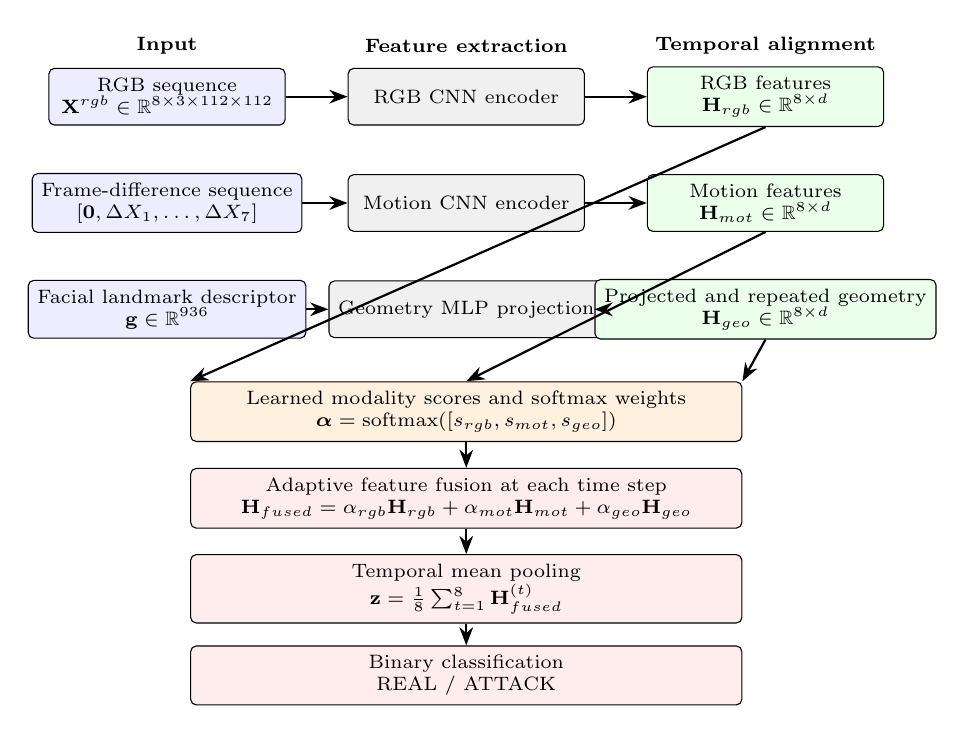
\begin{tikzpicture}[
    >=Stealth,
    input/.style={
        draw, rounded corners=2pt,
        fill=blue!7,
        minimum width=3.0cm,
        minimum height=0.72cm,
        align=center,
        font=\scriptsize
    },
    encoder/.style={
        draw, rounded corners=2pt,
        fill=gray!12,
        minimum width=3.0cm,
        minimum height=0.72cm,
        align=center,
        font=\scriptsize
    },
    feature/.style={
        draw, rounded corners=2pt,
        fill=green!8,
        minimum width=3.0cm,
        minimum height=0.72cm,
        align=center,
        font=\scriptsize
    },
    fusion/.style={
        draw, rounded corners=2pt,
        fill=orange!12,
        minimum width=7.0cm,
        minimum height=0.75cm,
        align=center,
        font=\scriptsize
    },
    output/.style={
        draw, rounded corners=2pt,
        fill=red!7,
        minimum width=7.0cm,
        minimum height=0.72cm,
        align=center,
        font=\scriptsize
    },
    arrow/.style={->, thick}
]

% Column headings
\node[font=\scriptsize\bfseries] at (0,0.65)
    {Input};
\node[font=\scriptsize\bfseries] at (3.8,0.65)
    {Feature extraction};
\node[font=\scriptsize\bfseries] at (7.6,0.65)
    {Temporal alignment};

% RGB branch
\node[input] (rgb_in) at (0,0)
    {RGB sequence\\
    $\mathbf{X}^{rgb}\in\mathbb{R}^{8\times 3\times112\times112}$};

\node[encoder] (rgb_enc) at (3.8,0)
    {RGB CNN encoder};

\node[feature] (rgb_feat) at (7.6,0)
    {RGB features\\
    $\mathbf{H}_{rgb}\in\mathbb{R}^{8\times d}$};

% Motion branch
\node[input] (mot_in) at (0,-1.35)
    {Frame-difference sequence\\
    $[\mathbf{0},\Delta X_1,\ldots,\Delta X_7]$};

\node[encoder] (mot_enc) at (3.8,-1.35)
    {Motion CNN encoder};

\node[feature] (mot_feat) at (7.6,-1.35)
    {Motion features\\
    $\mathbf{H}_{mot}\in\mathbb{R}^{8\times d}$};

% Geometry branch
\node[input] (geo_in) at (0,-2.7)
    {Facial landmark descriptor\\
    $\mathbf{g}\in\mathbb{R}^{936}$};

\node[encoder] (geo_enc) at (3.8,-2.7)
    {Geometry MLP projection};

\node[feature] (geo_feat) at (7.6,-2.7)
    {Projected and repeated geometry\\
    $\mathbf{H}_{geo}\in\mathbb{R}^{8\times d}$};

% Branch connections
\draw[arrow] (rgb_in) -- (rgb_enc);
\draw[arrow] (rgb_enc) -- (rgb_feat);

\draw[arrow] (mot_in) -- (mot_enc);
\draw[arrow] (mot_enc) -- (mot_feat);

\draw[arrow] (geo_in) -- (geo_enc);
\draw[arrow] (geo_enc) -- (geo_feat);

% Adaptive weighting
\node[fusion] (gates) at (3.8,-4.0)
    {Learned modality scores and softmax weights\\
    $\boldsymbol{\alpha}
    =\operatorname{softmax}([s_{rgb},s_{mot},s_{geo}])$};

\draw[arrow] (rgb_feat.south) -- (gates.north west);
\draw[arrow] (mot_feat.south) -- (gates.north);
\draw[arrow] (geo_feat.south) -- (gates.north east);

% Weighted fusion
\node[output] (weighted) at (3.8,-5.1)
    {Adaptive feature fusion at each time step\\
    $\mathbf{H}_{fused}
    =\alpha_{rgb}\mathbf{H}_{rgb}
    +\alpha_{mot}\mathbf{H}_{mot}
    +\alpha_{geo}\mathbf{H}_{geo}$};

\draw[arrow] (gates) -- (weighted);

% Temporal mean pooling
\node[output] (pool) at (3.8,-6.25)
    {Temporal mean pooling\\
    $\mathbf{z}=\frac{1}{8}\sum_{t=1}^{8}
    \mathbf{H}_{fused}^{(t)}$};

\draw[arrow] (weighted) -- (pool);

% Classification
\node[output] (classifier) at (3.8,-7.35)
    {Binary classification\\
    REAL / ATTACK};

\draw[arrow] (pool) -- (classifier);

\end{tikzpicture}%
}
\caption{Architecture of the E6 adaptive multi-cue feature
fusion model. RGB, motion, and facial geometry features are
temporally aligned, adaptively weighted, and aggregated
through temporal mean pooling before binary classification.}
\label{fig:e6_architecture}
\end{figure}


\subsection{Metrics}
Attack is the positive class. APCER is computed separately for each attack species; BPCER is the proportion of bona fide presentations classified as attacks. We define $\mathrm{APCER}_{max}=\max_s\mathrm{APCER}_s$ and
\begin{equation}
\mathrm{ACER}_{species}=\frac{\mathrm{APCER}_{max}+\mathrm{BPCER}}{2}.
\end{equation}
Accuracy, precision, recall, and F1-score use standard confusion-matrix definitions \cite{sokolova2009}. This species-aware definition is explicit and differs from a pooled APCER over all attacks.

\section{Results and Discussion}
\subsection{Test-set comparison}
Table~\ref{tab:results} reports results at validation-selected thresholds. E5 obtains the highest accuracy and F1-score; E6 obtains the lowest BPCER and species-aware ACER. E5 correctly classifies 966 sequences and E6 classifies 964, a difference of only two test sequences; this is not evidence of statistically established superiority.

\begin{table*}[t]
\caption{Test-set results at validation-selected thresholds (percent)}\label{tab:results}\centering\footnotesize
\begin{tabular}{lrrrrrrrr}\toprule
Model & $\tau$ & Acc. & Prec. & Recall & F1 & Max APCER & BPCER & ACER\\\midrule
E1 & .11 & 92.02 & 93.18 & 96.34 & 94.74 & 6.54 & 20.69 & 13.62\\
E2 & .82 & 88.41 & 95.24 & 88.90 & 91.96 & 24.77 & 13.03 & 18.90\\
E3 & .24 & 92.79 & 95.41 & 94.91 & 95.16 & 11.68 & 13.41 & 12.55\\
E4 & .04 & 92.79 & 92.20 & 98.69 & 95.33 & 2.80 & 24.52 & 13.66\\
E5 & .05 & \textbf{94.06} & 93.57 & 98.83 & \textbf{96.13} & \textbf{1.83} & 19.92 & 10.88\\
E6 & .33 & 93.87 & \textbf{96.43} & 95.30 & 95.86 & 8.41 & \textbf{10.34} & \textbf{9.38}\\
\bottomrule\end{tabular}
\end{table*}

E5 has the lowest maximum species APCER (1.83\%) but BPCER of 19.92\%. E6 has maximum APCER of 8.41\% but BPCER of 10.34\%, yielding the lowest species-aware ACER (9.38\%). Model selection is therefore metric-dependent: E5 is preferable when minimizing worst-species attack acceptance is prioritized, while E6 has the more favorable observed bona fide error and ACER.

\begin{table}[t]
\caption{Species-level APCER (percent)}\label{tab:species}\centering\footnotesize
\begin{tabular}{lrrr}\toprule
Model & iPad replay & iPhone replay & Printed photo\\\midrule
E1 & 2.51 & 2.56 & 6.54\\
E2 & 9.32 & 2.20 & 24.77\\
E3 & 2.51 & 2.56 & 11.68\\
E4 & 0.00 & 1.47 & 2.80\\
E5 & 1.43 & 1.83 & 0.00\\
E6 & 2.15 & 4.40 & 8.41\\
\bottomrule\end{tabular}
\end{table}

\subsection{Uncertainty and paired comparison}
A subject-level cluster bootstrap resampled the 20 test subjects with replacement, retaining all sequence observations for each sampled subject. It used 20,000 replicates, fixed validation thresholds, and percentile 95\% intervals. ACER intervals were E1 7.46--22.04\%, E2 12.51--25.81\%, E3 6.77--19.26\%, E4 6.80--22.58\%, E5 6.17--16.63\%, and E6 3.91--17.84\%. In the paired subject bootstrap, E5 minus E6 accuracy was +0.19 percentage points (95\% CI: -2.84 to +3.38) and ACER difference was +1.50 points (CI: -4.60 to +6.88); both intervals include zero. E5 had lower maximum APCER by 6.58 points (CI: -14.14 to -1.43), while E6 had lower BPCER by 9.58 points (E5 minus E6 CI: +1.93 to +18.04). These intervals quantify test-subject sampling conditional on seed-42 checkpoints, not training-seed variability.

\subsection{Web application implementation}
The trained E6 checkpoint is integrated into a browser-facing application that captures an eight-frame camera sequence and sends it to a prediction API. The web interface presents the predicted class and class probabilities. Fig.~\ref{fig:webapp} shows the original example result screen from the running application. The displayed ATTACK decision and probabilities are illustrative output from one capture, not an independent accuracy measurement. Offline test metrics and API timing are reported separately.

\begin{figure}[t]
    \centering
    \includegraphics[width=\columnwidth]{web_liveness_result.png}
    \caption{Browser interface of the web-based liveness detection application using the E6 adaptive RGB--motion--geometry model.}
    \label{fig:webapp}
\end{figure}

\subsection{API latency}
The E6 endpoint was benchmarked with five warm-up requests followed by 50 measured sequential HTTP requests; all succeeded. Mean latency was 190.498 ms, median 175.181 ms, and P95 284.893 ms. The reciprocal of mean sequential latency is 5.247 requests/s. This is a sequential-equivalent rate, not concurrent throughput or server capacity. Payload encoding and dataset disk reads were excluded. Previously reported very small RSS and zero-CPU samples are omitted because they do not provide a reliable estimate of total inference-process resource use. GPU/VRAM was not measured.

\begin{table}[t]
\caption{E6 sequential API benchmark}\label{tab:latency}\centering\footnotesize
\begin{tabular}{lr}\toprule
Metric & Result\\\midrule
Warm-up / measured requests & 5 / 50\\
Successful / failed & 50 / 0\\
Mean latency & 190.498 ms\\
Median latency (P50) & 175.181 ms\\
P95 latency & 284.893 ms\\
Minimum / maximum & 151.352 / 340.002 ms\\
Reciprocal mean latency & 5.247 requests/s\\
Concurrent capacity & Not measured\\
GPU / VRAM & Not measured\\\bottomrule
\end{tabular}
\end{table}

\subsection{Limitations}
The study uses one processed dataset, one subject-disjoint split, and one training seed. It does not establish cross-dataset generalization. Geometry filtering excludes 42 REAL training sequences, changing the training distribution and confounding geometry comparisons. The validation set contains three subjects. The test set includes three attack species, and missing-geometry test-time handling was not assessed because all test sequences had eight valid frames. Repeated-seed experiments, external-dataset evaluation, and concurrent load testing remain future work.

\section{Conclusion}
This study investigated six face liveness detection configurations by integrating RGB appearance, frame-difference motion, and facial geometry features. Experimental results demonstrate that different feature combinations produce distinct classification and presentation attack detection characteristics. E5 achieved the highest accuracy (94.06\%) and the lowest maximum species APCER (1.83\%), whereas E6, which incorporates adaptive modality weighting and temporal mean pooling, achieved the lowest BPCER (10.34\%) and species-aware ACER (9.38\%). These findings highlight the potential of adaptive multi-cue fusion to balance bona fide presentation detection and presentation attack detection. However, subject-level paired bootstrap analysis did not establish a statistically reliable difference in accuracy or ACER between E5 and E6. Consequently, selecting between these configurations should consider the operational security requirements and the relative costs of accepting presentation attacks and rejecting bona fide users, rather than relying on accuracy alone. Despite these findings, the evaluation is limited to a single subject-disjoint MSU-MFSD split and seed-42 checkpoints. Future work will investigate cross-dataset generalization, repeated-seed evaluation, improved handling of invalid facial geometry, and optimization under concurrent inference workloads to establish the robustness and deployment scalability of the proposed system.


\FloatBarrier
\begin{thebibliography}{00}
\bibitem{wen2015ida} D. Wen, H. Han, and A. K. Jain, ``Face Spoof Detection With Image Distortion Analysis,'' \emph{IEEE Transactions on Information Forensics and Security}, vol. 10, no. 4, pp. 746--761, Apr. 2015, doi: 10.1109/TIFS.2015.2400395.
\bibitem{yu2023survey} Z. Yu, Y. Qin, X. Li, C. Zhao, Z. Lei, and G. Zhao, ``Deep Learning for Face Anti-Spoofing: A Survey,'' \emph{IEEE Transactions on Pattern Analysis and Machine Intelligence}, vol. 45, no. 5, pp. 5609--5631, May 2023, doi: 10.1109/TPAMI.2022.3215850.
\bibitem{liu2018aux} Y. Liu, A. Jourabloo, and X. Liu, ``Learning Deep Models for Face Anti-Spoofing: Binary or Auxiliary Supervision,'' in \emph{Proc. IEEE CVPR}, 2018, pp. 389--398.
\bibitem{yu2020cdcn} Z. Yu \emph{et al.}, ``Searching Central Difference Convolutional Networks for Face Anti-Spoofing,'' in \emph{Proc. IEEE/CVF CVPR}, 2020, pp. 5295--5305, doi: 10.1109/CVPR42600.2020.00534.
\bibitem{yang2019stasn} X. Yang \emph{et al.}, ``Face Anti-Spoofing: Model Matters, so Does Data,'' in \emph{Proc. IEEE/CVF CVPR}, 2019, pp. 3507--3516.
\bibitem{sun2018temporal} Z. Sun, L. Sun, and Q. Li, ``Investigation in Spatial-Temporal Domain for Face Spoof Detection,'' in \emph{Proc. IEEE ICASSP}, 2018.
\bibitem{silva2023spatiotemporal} V. L. da Silva \emph{et al.}, ``Residual Spatiotemporal Convolutional Networks for Face Anti-Spoofing,'' \emph{Journal of Visual Communication and Image Representation}, vol. 91, Art. no. 103744, 2023, doi: 10.1016/j.jvcir.2022.103744.
\bibitem{chang2023geometry} C.-J. Chang \emph{et al.}, ``A Closer Look at Geometric Temporal Dynamics for Face Anti-Spoofing,'' in \emph{Proc. IEEE/CVF CVPR Workshops}, 2023, pp. 1081--1091, doi: 10.1109/CVPRW59228.2023.00115.
\bibitem{shen2019facebagnet} T. Shen, Y. Huang, and Z. Tong, ``FaceBagNet: Bag-Of-Local-Features Model for Multi-Modal Face Anti-Spoofing,'' in \emph{Proc. IEEE/CVF CVPR Workshops}, 2019.
\bibitem{yu2020multimodal} Z. Yu \emph{et al.}, ``Multi-Modal Face Anti-Spoofing Based on Central Difference Networks,'' in \emph{Proc. IEEE/CVF CVPR Workshops}, 2020, pp. 2766--2774, doi: 10.1109/CVPRW50498.2020.00333.
\bibitem{chen2025mmfas} G. Chen \emph{et al.}, ``mmFAS: Multimodal Face Anti-Spoofing Using Multi-Level Alignment and Switch-Attention Fusion,'' in \emph{Proc. AAAI}, vol. 39, no. 1, pp. 58--66, 2025, doi: 10.1609/aaai.v39i1.31980.
\bibitem{zeng2023bandpass} D. Zeng \emph{et al.}, ``Bandpass Filter Based Dual-Stream Network for Face Anti-Spoofing,'' in \emph{Proc. IEEE/CVF CVPR Workshops}, 2023, pp. 6403--6410.
\bibitem{kagglemsumfsd} minhtranv, ``MSU-MFSD Processed into Frames,'' Kaggle dataset, accessed Oct. 2026. [Online]. Available: \url{https://www.kaggle.com/datasets/minhtranv/msu-mfsd-processed-into-frames}.
\bibitem{sokolova2009} M. Sokolova and G. Lapalme, ``A systematic analysis of performance measures for classification tasks,'' \emph{Information Processing \& Management}, vol. 45, no. 4, pp. 427--437, 2009, doi: 10.1016/j.ipm.2009.03.002.
\bibitem{iso30107} ISO/IEC, \emph{ISO/IEC 30107-3:2023 Information Technology---Biometric Presentation Attack Detection---Part 3: Testing and Reporting}. Geneva, Switzerland: International Organization for Standardization, 2023.
\end{thebibliography}
\end{document}
